\documentclass[usenames,dvipsnames]{beamer}
\usetheme{Berlin}
\usepackage[utf8]{inputenc}
\usepackage[english]{babel}
\usepackage{graphicx}
\usepackage{url}
\usepackage{multicol}
\usepackage{relsize}
\usepackage{enumitem}
\usepackage{fancyvrb}

\graphicspath{ {images/} }

\title{Secure memory handling in C}
\subtitle{}
\author{Alexander Livenets \\ Oliver Esser}
\institute{}
\date{25 June 2019}

\newcommand{\codeinline}[1] {\texttt{\smaller[2]{#1}}}

\begin{document}

\AtBeginSection[]
{
\begin{frame}
\frametitle{Table of Contents}
\tableofcontents[currentsection]
\end{frame}
}

\setbeamertemplate{endpage}{%
\begin{frame}
\center \Huge Thanks!
\end{frame}
}

\begin{frame}
\titlepage
\end{frame}

\section{Memory handling}
\begin{frame}[fragile]
\frametitle{Buffer overflow example}
\tiny
\begin{verbatim}
int copy_string(const char *s) {
char buffer[64];
strcpy(buffer, s);
}

int main(void) {
char large_string[128] = "Hello World!";
copy_string(large_string); //OK...

// Fill large string
for(int i = 0; i < sizeof(large_string) - 1; ++i)
large_string[i] = 'a';
large_string[sizeof(large_string) - 1] = '\0';

copy_string(large_string); // Buffer overflow...
}
\end{verbatim}
\note{When string on stack overflows, return address or other sensitive data on stack may be corrupted, hence allowing to perform attack}
\end{frame}

\begin{frame}
\centering
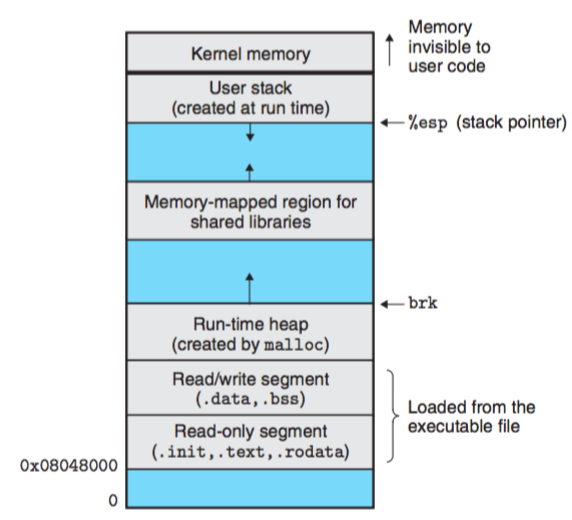
\includegraphics[scale=0.35]{linux_mem.png}

\tiny{\url{https://people.cs.pitt.edu/~xianeizhang/notes/Linking.html}}
\end{frame}

\begin{frame}
\centering
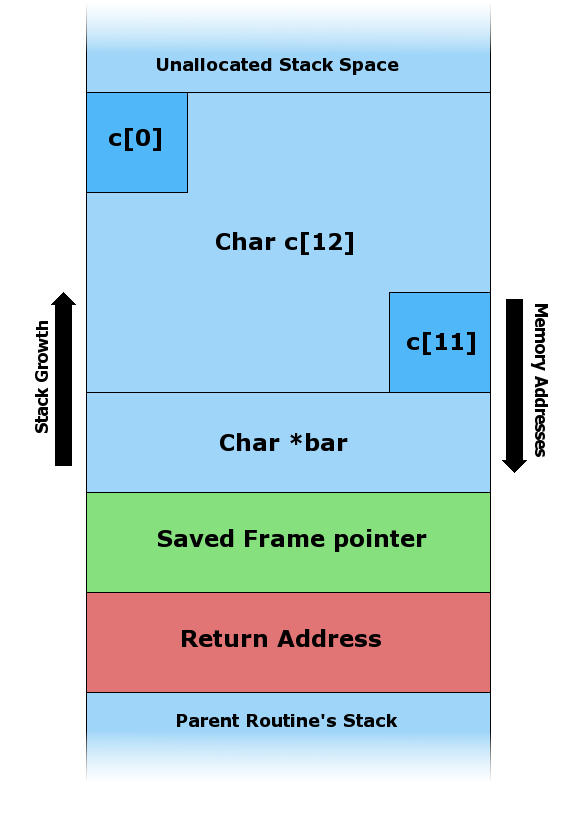
\includegraphics[scale=0.16]{Stack_Overflow_2.png}
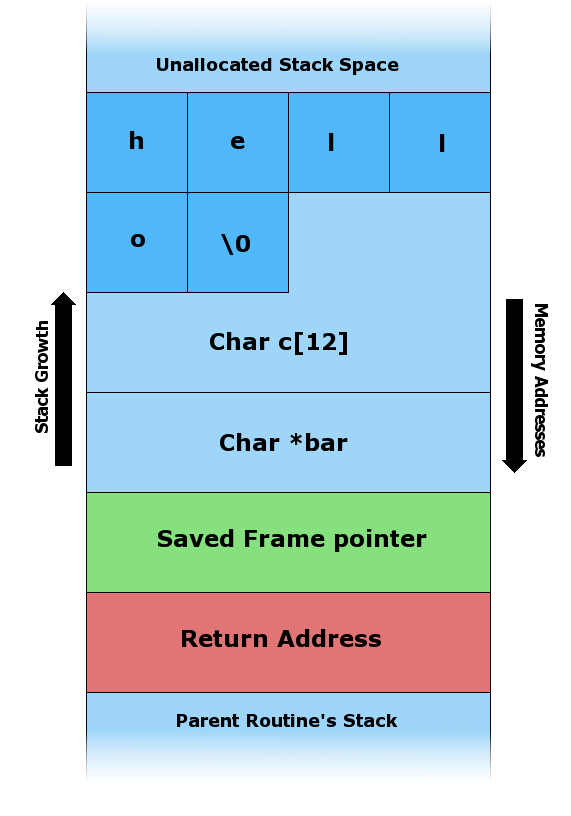
\includegraphics[scale=0.16]{Stack_Overflow_3.png}
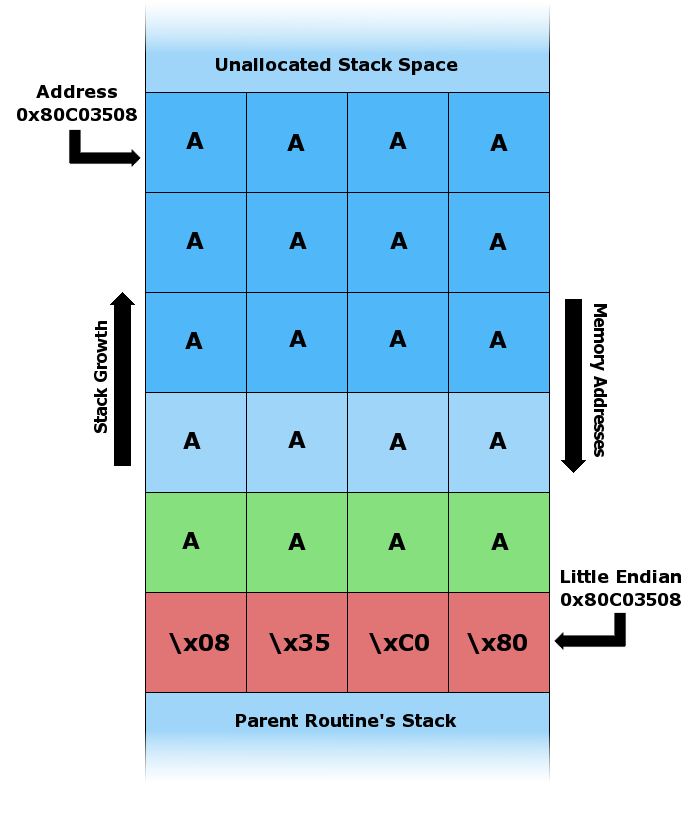
\includegraphics[scale=0.16]{Stack_Overflow_4.png}

\tiny{\url{https://en.wikipedia.org/wiki/Stack_buffer_overflow}}

\note{Show results of buffer overflow: return address may be overwritten and function will return to the malicious address}
\end{frame}

\section{strcpy family}
\subsection{libc}
\begin{frame}[fragile]
\frametitle{\secname}
\begin{itemize}[label={},leftmargin=*]
\item \codeinline{char *strcpy(char *dst, const char *src);}
\item \codeinline{char *strncpy(char *dst, const char *src, size\_t dst\_size);}
\item \codeinline{char *strcat(char *dst, const char *src);}
\item \codeinline{char *strncat(char *dst, const char *src, size\_t dst\_size);} TODO: write examples
\end{itemize}

\par
\codeinline{man strcpy, BUGS section:}
\tiny
\begin{Verbatim}[commandchars=\\\{\}]
If the destination string of a strcpy() is not large enough, then anything might happen.
Overflowing fixed-length string buffers is a favorite cracker technique for taking complete
control of the machine. Any time a program reads or copies data into a buffer, the program
first needs to check that there's enough space. This may be unnecessary if you can show that
overflow is impossible, but be careful: \textbf{programs can get changed over time},
in ways that may make the impossible possible.
\end{Verbatim}

\end{frame}

\subsection{libbsd}
\begin{frame}
\frametitle{\secname}
\codeinline{libbsd:}
\begin{itemize}[label={},leftmargin=*]
\item \codeinline{size\_t strlcpy(char *dst, const char *src, size\_t dst\_size);}
\item \codeinline{size\_t strlcat(char *dst, const char *src, size\_t dst\_size);}
\end{itemize}

\end{frame}

\section{sprintf family}
\begin{frame}
\begin{itemize}[label={},leftmargin=*]
\item \codeinline{int sprintf(char *str, char *fmt, ...);}
\item \codeinline{int snprintf(char *str, size\_t len, char *fmt, ...);}
\end{itemize}
\end{frame}

\section{Good practices}
\subsection{Compiler tricks and tips}
\begin{frame}
\frametitle{\subsecname}
\small
GCC compiler parameters:
\begin{itemize}[leftmargin=*]
	\setlength\itemsep{0.3em}
	\item \codeinline{-Wformat=\{1,2\} -Wformat-nonliteral -Wformat-overflow -Wformat-signedness -Wformat-y2k -Wformat-security -Wformat-nonliteral}
	\item \codeinline{-Wformat-truncation=\{1,2\}}
	\item \codeinline{-Wstringop-overflow=\{1,2,3,4\}}
	\item \codeinline{-Wstringop-truncation}
	\item \codeinline{-Warray-bounds=\{1,2\}}
\end{itemize}

GCC instrumentation options:
\begin{itemize}[leftmargin=*]
	\setlength\itemsep{0.3em}
	\item \codeinline{-fstack-protector-\{all,strong,explicit,\}}
	\item \codeinline{-fsanitize=address}
	\item \codeinline{-fsanitize=undefined -fsanitize=null -fsanitize=bounds -fsanitize=bounds-strict}
	\item \codeinline{-fsanitize=pointer-compare -fsanitize=pointer-subtract}
	\item \codeinline{-fsanitize=pointer-overflow}
	\item \codeinline{-fsanitize-address-use-after-scope}
	\item \codeinline{\_\_attribute\_\_ ((format (printf, 2, 3)))}
\end{itemize}
\end{frame}

\subsection{Recommendations}
\begin{frame}
\frametitle{\subsecname}
\begin{itemize}[leftmargin=*]
	\item C: Use C >= C99(best, use C11)
	\item C: use function accepting buffer size parameter: \codeinline{strn\*}: \codeinline{strncpy, strnlen,...}
	\item C APIs: write C++ API wrappers
	\item C++: use \codeinline{std::ostringstream}
	\item C++: \codeinline{std::string}, \codeinline{std::string\_view} (C++17)
	\item When writing functions, pass max. buffer size in function, e.g.: \codeinline{void f(char *s, size\_t len);}
	\item Use \codeinline{snprintf} to copy strings
	\item Validate input data from external sources
	\item Common: Secure Coding Practices, Safe Coding Practices
\end{itemize}
\end{frame}

\section{References}
\begin{frame}
\frametitle{\secname}
\footnotesize
\begin{itemize}[leftmargin=*]
	\item \url{https://people.cs.pitt.edu/~xianeizhang/notes/Linking.html}
	\item \url{https://safecode.org/courses/secure-memory-handling-in-c-101/}
\end{itemize}
\end{frame}

\usebeamertemplate{endpage}

\end{document}
